\chapter{Listings}

\lstset{language=Java}
\lstinputlisting[captionpos=b,label={app:feedbacks},caption={Die Liste von Benutzerfeedbacks}]{Listings/feedbacks.json}

\lstset{language=Java}
\lstinputlisting[captionpos=b,label={app:pigcorpus},caption={Erzeugung eines Wikipedia-Korpus}]{Listings/pig.java}

\lstset{language=Java}
\lstinputlisting[captionpos=b,label={app:trainonlp},caption={Training eines ME-Modells (OpenNLP)}]{Listings/train-onlp.java}

\lstset{language=python}
\lstinputlisting[captionpos=b,label={app:trainmitie},caption={Training eines ME-Modells (OpenNLP)}]{Listings/train-mitie.py}

%\clearpage
%\chapter{Tabellen}

\clearpage
\chapter{Screenshots}

\begin{figure}
\centering
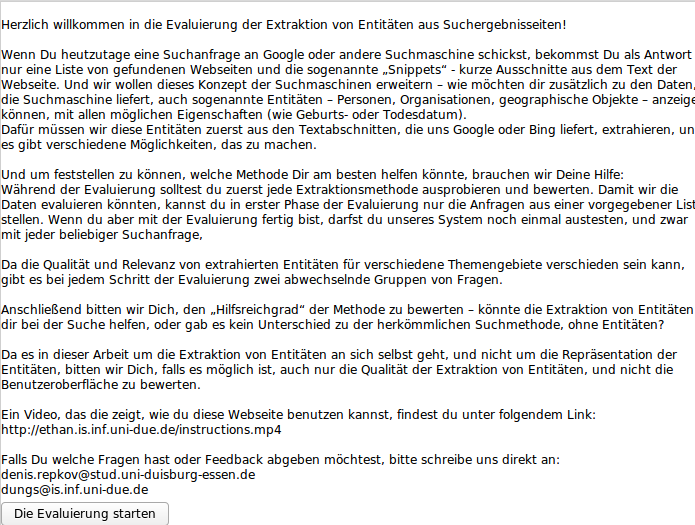
\includegraphics[width=1.0\textwidth]{Bilder/evalstep01.png}
\caption{''Einleitung in die Evaluierung''}
\label{app:evalstep01}
\end{figure}

\begin{figure}
\centering
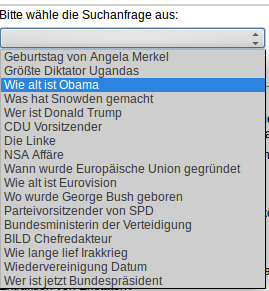
\includegraphics[width=.6\textwidth]{Bilder/select-question.png}
\caption{''Auswahl einer Frage''}
\label{fig:eval-select-question}
\end{figure}

\begin{figure}
\centering
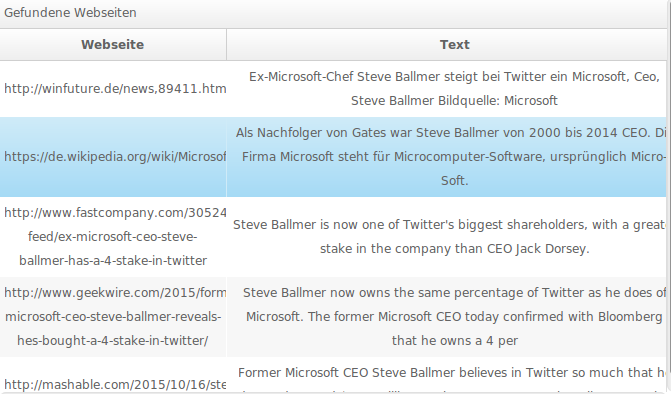
\includegraphics[width=1\textwidth]{Bilder/evalstep02-step1.png}
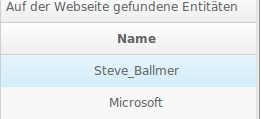
\includegraphics[width=0.5\textwidth]{Bilder/evalstep02-step1-2.png}
\caption{''Liste von Snippets und gefundenen Entitäten''}
\label{fig:eval-entitylist}
\end{figure}

\begin{figure}
\centering
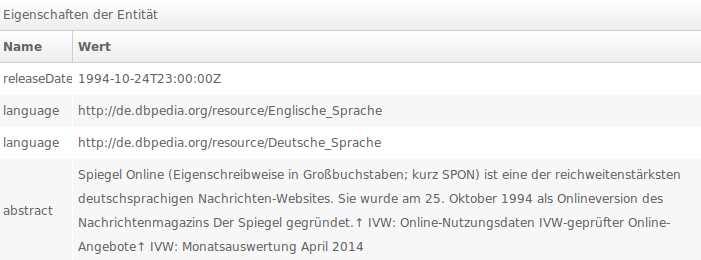
\includegraphics[width=1\textwidth]{Bilder/eval-step03.png}
\caption{''Liste von Eigenschaften einer Entität''}
\label{fig:eval-props}
\end{figure}

\begin{figure}
\centering
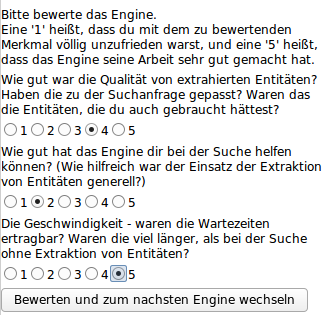
\includegraphics[width=0.6\textwidth]{Bilder/bewertung-eval.png}
\caption{''Bewertung eines Engines''}
\label{fig:bewertung}
\end{figure}

\begin{figure}
\centering
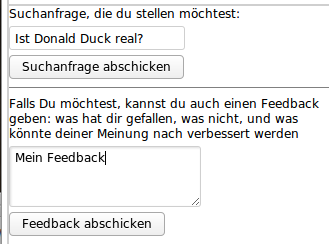
\includegraphics[width=0.6\textwidth]{Bilder/ende-eval-01.png}
\caption{''Eingabeform des letzten Evaluierungsschritt''}
\label{fig:finish-eval}
\end{figure}
